\chapter{Introduction au Texte et aux S\'eries Temporelles}
\label{ch:texte_temporel}

\section{Donn\'ees textuelles}
\label{sec:donnees_textuelles}

\index{donn\'ees textuelles}\index{NLP}

\begin{definition}[Traitement automatique du langage]
Le \textbf{traitement automatique du langage naturel}\index{traitement automatique du langage} (\textit{Natural Language Processing}, NLP) regroupe les techniques permettant aux machines de comprendre et manipuler du texte. Pour utiliser du texte en apprentissage automatique, il faut le convertir en \textbf{repr\'esentation num\'erique}.
\end{definition}

\subsection{Sac de mots (\textit{Bag of Words})}

\index{sac de mots}\index{bag of words}\index{CountVectorizer}

\begin{definition}[Sac de mots]
Le mod\`ele \textbf{sac de mots} repr\'esente chaque document comme un vecteur de fr\'equences de mots, en ignorant l'ordre et la grammaire.
\end{definition}

\begin{center}
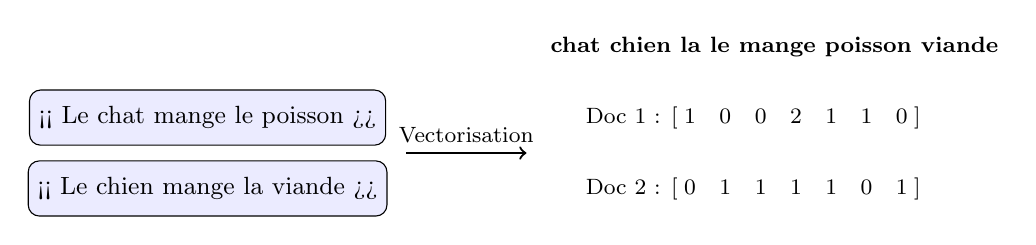
\begin{tikzpicture}[scale=0.9]
    % Documents
    \node[draw, rounded corners, fill=blue!8, minimum width=4cm, minimum height=0.7cm, font=\small] (d1) at (0, 2) {<<~Le chat mange le poisson~>>};
    \node[draw, rounded corners, fill=blue!8, minimum width=4cm, minimum height=0.7cm, font=\small] (d2) at (0, 1) {<<~Le chien mange la viande~>>};

    % Fl\`eche
    \draw[->, thick] (2.8, 1.5) -- (4.5, 1.5) node[midway, above, font=\footnotesize] {Vectorisation};

    % Matrice
    \node[font=\footnotesize\bfseries] at (8, 3) {chat chien la le mange poisson viande};
    \node[font=\footnotesize, anchor=west] at (5.2, 2) {Doc 1~: $[\;1\quad 0\quad 0\quad 2\quad 1\quad 1\quad 0\;]$};
    \node[font=\footnotesize, anchor=west] at (5.2, 1) {Doc 2~: $[\;0\quad 1\quad 1\quad 1\quad 1\quad 0\quad 1\;]$};
\end{tikzpicture}
\end{center}

\begin{codeblock}[title=\textbf{Python}]
\begin{minted}{python}
from sklearn.feature_extraction.text import CountVectorizer

documents = [
    "Le chat mange le poisson",
    "Le chien mange la viande",
    "Le chat et le chien jouent"
]

vectorizer = CountVectorizer()
X = vectorizer.fit_transform(documents)

print("Vocabulaire :", vectorizer.get_feature_names_out())
print()
print("Matrice document-terme :")
print(X.toarray())
\end{minted}
\end{codeblock}

\begin{codeoutput}
\begin{minted}{text}
Vocabulaire : ['chat' 'chien' 'et' 'jouent' 'la' 'le' 'mange' 'poisson' 'viande']

Matrice document-terme :
[[1 0 0 0 0 2 1 1 0]
 [0 1 0 0 1 1 1 0 1]
 [1 1 1 1 0 2 0 0 0]]
\end{minted}
\end{codeoutput}

\subsection{TF-IDF}

\index{TF-IDF}\index{TfidfVectorizer}

\begin{definition}[TF-IDF]
\textbf{TF-IDF}\index{TF-IDF} (\textit{Term Frequency--Inverse Document Frequency}) pond\`ere chaque terme par son importance~:
\[
\text{TF-IDF}(t, d) = \text{TF}(t, d) \times \text{IDF}(t)
\]
o\`u $\text{TF}(t,d)$ est la fr\'equence du terme $t$ dans le document $d$ et~:
\[
\text{IDF}(t) = \log\frac{n_{\text{docs}}}{n_{\text{docs contenant } t}}
\]
Les mots fr\'equents partout (comme <<~le ~>>) re\c{c}oivent un poids faible.
\end{definition}

\begin{codeblock}[title=\textbf{Python}]
\begin{minted}{python}
from sklearn.feature_extraction.text import TfidfVectorizer
import numpy as np

tfidf = TfidfVectorizer()
X_tfidf = tfidf.fit_transform(documents)

print("Vocabulaire :", tfidf.get_feature_names_out())
print()
print("Matrice TF-IDF (arrondie) :")
print(np.round(X_tfidf.toarray(), 2))
\end{minted}
\end{codeblock}

\begin{codeoutput}
\begin{minted}{text}
Vocabulaire : ['chat' 'chien' 'et' 'jouent' 'la' 'le' 'mange' 'poisson' 'viande']

Matrice TF-IDF (arrondie) :
[[0.35 0.   0.   0.   0.   0.55 0.35 0.46 0.  ]
 [0.   0.35 0.   0.   0.46 0.28 0.35 0.   0.46]
 [0.31 0.31 0.41 0.41 0.   0.49 0.   0.   0.  ]]
\end{minted}
\end{codeoutput}

\begin{intuition}
Les mots <<~poisson ~>> et <<~viande ~>> ont des poids TF-IDF \'elev\'es car ils sont \textbf{discriminants}~: ils n'apparaissent que dans un seul document. Le mot <<~le ~>>, pr\'esent partout, a un poids relativement plus faible.
\end{intuition}

\subsection{Classification de texte}

\begin{codeblock}[title=\textbf{Python}]
\begin{minted}{python}
from sklearn.datasets import fetch_20newsgroups
from sklearn.feature_extraction.text import TfidfVectorizer
from sklearn.naive_bayes import MultinomialNB
from sklearn.pipeline import Pipeline
from sklearn.metrics import classification_report

# Sous-ensemble de 4 cat\'egories
categories = ['sci.space', 'comp.graphics', 'rec.sport.baseball', 'talk.politics.misc']

train = fetch_20newsgroups(subset='train', categories=categories, random_state=42)
test = fetch_20newsgroups(subset='test', categories=categories, random_state=42)

# Pipeline : TF-IDF + Naive Bayes
pipeline = Pipeline([
    ('tfidf', TfidfVectorizer(max_features=5000, stop_words='english')),
    ('clf', MultinomialNB())
])

pipeline.fit(train.data, train.target)
y_pred = pipeline.predict(test.data)

print(classification_report(test.target, y_pred,
                            target_names=train.target_names))
\end{minted}
\end{codeblock}

\begin{codeoutput}
\begin{minted}{text}
                    precision    recall  f1-score   support

     comp.graphics       0.89      0.88      0.89       389
  rec.sport.baseball       0.96      0.94      0.95       397
           sci.space       0.92      0.91      0.91       394
  talk.politics.misc       0.82      0.85      0.83       310

          accuracy                           0.90      1490
         macro avg       0.90      0.90      0.90      1490
      weighted avg       0.90      0.90      0.90      1490
\end{minted}
\end{codeoutput}

\begin{bonnepratique}
Utilisez \py{Pipeline} pour cha\^iner le pr\'etraitement et le mod\`ele. Cela garantit que la vectorisation est apprise uniquement sur les donn\'ees d'entra\^inement, \'evitant les fuites de donn\'ees (\textit{data leakage})\index{fuite de donn\'ees}.
\end{bonnepratique}

\section{S\'eries temporelles}
\label{sec:series_temporelles}

\index{s\'erie temporelle}

\begin{definition}[S\'erie temporelle]
Une \textbf{s\'erie temporelle} est une suite d'observations $(y_{t_1}, y_{t_2}, \ldots, y_{t_n})$ index\'ees par le temps. L'analyse des s\'eries temporelles vise \`a comprendre les tendances, la saisonnalit\'e et \`a effectuer des pr\'evisions.
\end{definition}

\subsection{Manipulation des dates avec pandas}

\index{datetime}\index{pd.to\_datetime}\index{resample}

\begin{codeblock}[title=\textbf{Python}]
\begin{minted}{python}
import pandas as pd
import numpy as np

# Cr\'eation d'une s\'erie temporelle (donn\'ees de type AirPassengers)
np.random.seed(42)
dates = pd.date_range(start='1949-01', periods=144, freq='MS')
trend = np.linspace(100, 500, 144)
seasonal = 40 * np.sin(2 * np.pi * np.arange(144) / 12)
noise = np.random.normal(0, 10, 144)
passengers = trend + seasonal + noise

ts = pd.Series(passengers, index=dates, name='passengers')
print(ts.head(12))
print(f"\nType d'index : {type(ts.index)}")
\end{minted}
\end{codeblock}

\begin{codeoutput}
\begin{minted}{text}
1949-01-01    105.0
1949-02-01    118.2
1949-03-01    139.4
1949-04-01    147.8
1949-05-01    141.9
1949-06-01    127.2
1949-07-01    110.3
1949-08-01     96.7
1949-09-01     88.4
1949-10-01     92.4
1949-11-01    107.5
1949-12-01    124.1
Freq: MS, Name: passengers, dtype: float64

Type d'index : <class 'pandas.core.indexes.datetimes.DatetimeIndex'>
\end{minted}
\end{codeoutput}

\subsection{L'accesseur \texttt{.dt}}

\begin{codeblock}[title=\textbf{Python}]
\begin{minted}{python}
df = pd.DataFrame({'date': dates, 'passengers': passengers})

# Extraction de composantes temporelles
df['annee'] = df['date'].dt.year
df['mois'] = df['date'].dt.month
df['jour_semaine'] = df['date'].dt.day_name()

print(df[['date', 'annee', 'mois', 'jour_semaine']].head())
\end{minted}
\end{codeblock}

\begin{codeoutput}
\begin{minted}{text}
        date  annee  mois jour_semaine
0 1949-01-01   1949     1     Saturday
1 1949-02-01   1949     2     Tuesday
2 1949-03-01   1949     3     Tuesday
3 1949-04-01   1949     4     Friday
4 1949-05-01   1949     5     Sunday
\end{minted}
\end{codeoutput}

\subsection{R\'e-\'echantillonnage et moyennes mobiles}

\index{r\'e-\'echantillonnage}\index{moyenne mobile}\index{rolling}

\begin{codeblock}[title=\textbf{Python}]
\begin{minted}{python}
# R\'e-\'echantillonnage annuel
annual = ts.resample('YE').mean()
print("Moyenne annuelle (5 premi\`eres ann\'ees) :")
print(annual.head().round(1))

# Moyenne mobile sur 12 mois
rolling_12 = ts.rolling(window=12).mean()
print("\nMoyenne mobile 12 mois (derni\`eres valeurs) :")
print(rolling_12.tail(5).round(1))
\end{minted}
\end{codeblock}

\begin{codeoutput}
\begin{minted}{text}
Moyenne annuelle (5 premi\`eres ann\'ees) :
1949-12-31    116.6
1950-12-31    149.7
1951-12-31    182.5
1952-12-31    215.5
1953-12-31    248.7
Freq: YE-DEC, Name: passengers, dtype: float64

Moyenne mobile 12 mois (derni\`eres valeurs) :
1960-08-01    460.4
1960-09-01    464.1
1960-10-01    467.2
1960-11-01    470.5
1960-12-01    473.0
Name: passengers, dtype: float64
\end{minted}
\end{codeoutput}

\subsection{D\'ecomposition d'une s\'erie temporelle}

\index{d\'ecomposition}\index{tendance}\index{saisonnalit\'e}\index{seasonal\_decompose}

\begin{definition}[D\'ecomposition]
Une s\'erie temporelle peut \^etre d\'ecompos\'ee en trois composantes~:
\[
y_t = T_t + S_t + R_t
\]
o\`u $T_t$ est la \textbf{tendance}\index{tendance}, $S_t$ la \textbf{saisonnalit\'e}\index{saisonnalit\'e} et $R_t$ le \textbf{r\'esidu}\index{r\'esidu}.
\end{definition}

\begin{codeblock}[title=\textbf{Python}]
\begin{minted}{python}
from statsmodels.tsa.seasonal import seasonal_decompose

# D\'ecomposition additive
decomposition = seasonal_decompose(ts, model='additive', period=12)

print("Composante tendance (12 premi\`eres valeurs) :")
print(decomposition.trend.dropna().head(6).round(1))
print("\nComposante saisonni\`ere (12 premi\`eres valeurs) :")
print(decomposition.seasonal.head(12).round(1))
\end{minted}
\end{codeblock}

\begin{codeoutput}
\begin{minted}{text}
Composante tendance (12 premi\`eres valeurs) :
1949-07-01    116.4
1949-08-01    119.0
1949-09-01    121.7
1949-10-01    124.4
1949-11-01    127.0
1949-12-01    129.7
Name: trend, dtype: float64

Composante saisonni\`ere (12 premi\`eres valeurs) :
1949-01-01    -7.3
1949-02-01     6.2
1949-03-01    22.8
1949-04-01    32.1
1949-05-01    27.3
1949-06-01    10.4
1949-07-01    -8.4
1949-08-01   -24.3
1949-09-01   -32.2
1949-10-01   -27.0
1949-11-01   -10.4
1949-12-01     6.5
Name: seasonal, dtype: float64
\end{minted}
\end{codeoutput}

\begin{remarque}
La d\'ecomposition peut \^etre \textbf{additive} ($y_t = T_t + S_t + R_t$) ou \textbf{multiplicative} ($y_t = T_t \times S_t \times R_t$). Le mod\`ele multiplicatif est adapt\'e lorsque l'amplitude de la saisonnalit\'e cro\^it avec la tendance.
\end{remarque}

\section{Exercices}

\begin{exercice}[$\star$]
Cr\'eez un \py{CountVectorizer} sur les phrases suivantes~: <<~J'aime le Python ~>>, <<~J'aime les statistiques ~>>, <<~Python et statistiques sont utiles ~>>. Affichez la matrice document-terme et le vocabulaire.
\end{exercice}

\begin{exercice}[$\star\star$]
Chargez le jeu de donn\'ees \py{fetch_20newsgroups} avec les cat\'egories \py{['sci.med', 'sci.electronics']}. Construisez un pipeline TF-IDF + r\'egression logistique. \'Evaluez avec la validation crois\'ee \`a 5 plis et affichez le rapport de classification.
\end{exercice}

\begin{exercice}[$\star\star$]
Cr\'eez une s\'erie temporelle quotidienne sur 3 ans avec une tendance lin\'eaire et une saisonnalit\'e hebdomadaire. R\'e-\'echantillonnez par semaine et par mois. Tracez les trois graphiques (quotidien, hebdomadaire, mensuel).
\end{exercice}

\begin{exercice}[$\star\star\star$]
Chargez un jeu de donn\'ees temporelles r\'eel (par exemple, les donn\'ees de temp\'erature de \py{statsmodels.datasets}). Appliquez la d\'ecomposition saisonni\`ere. Tracez les quatre composantes (s\'erie originale, tendance, saisonnalit\'e, r\'esidu) sur des sous-graphiques.
\end{exercice}

\begin{exercice}[$\star\star\star$]
Comparez les performances de classification de texte en utilisant (a) \py{CountVectorizer}, (b) \py{TfidfVectorizer} et (c) \py{TfidfVectorizer(ngram_range=(1,2))} sur le jeu 20 newsgroups (4 cat\'egories au choix). Utilisez un classifieur \py{MultinomialNB} et rapportez les exactitudes.
\end{exercice}

\begin{formules}
\textbf{R\'esum\'e du chapitre~\ref{ch:texte_temporel}}
\begin{itemize}
    \item \textbf{Sac de mots}~: \py{CountVectorizer()}, matrice de fr\'equences de termes.
    \item \textbf{TF-IDF}~: \py{TfidfVectorizer()}, $\text{TF-IDF}(t,d) = \text{TF}(t,d) \times \log\frac{n_{\text{docs}}}{n_{\text{docs}(t)}}$.
    \item \textbf{Pipeline}~: \py{Pipeline([('tfidf', TfidfVectorizer()), ('clf', ...)])}.
    \item \textbf{Dates pandas}~: \py{pd.to_datetime()}, accesseur \py{.dt} (year, month, day\_name).
    \item \textbf{R\'e-\'echantillonnage}~: \py{ts.resample('ME').mean()}.
    \item \textbf{Moyenne mobile}~: \py{ts.rolling(window=k).mean()}.
    \item \textbf{D\'ecomposition}~: $y_t = T_t + S_t + R_t$ via \py{seasonal_decompose()}.
\end{itemize}
\end{formules}
